\chapter{Конструкторская часть}
В данном разделе будут реализованы схемы алгоритмов умножения матриц, приведено описание используемых типов данных, а также описана структура программного обеспечения.

\section{Требования к программному обеспечению}\label{section:requirements_1}
К программе предъявлен ряд функциональных требований:
\begin{itemize}
    \item на вход подаются две матрицы;
    \item матрицы располагаются в файлах, с расширением \texttt{*.txt}.
    \item на выходе~--- матрица, являющаяся результатом умножения матриц.
\end{itemize}

К программе предъявлен ряд требований:
\begin{itemize}
	\item наличие интерфейса для выбора действия;
	\item наличие функциональных замеров процессорного времени выполнения алгоритмов умножения матриц;
	\item замеры процессорного времени выполнятся только для квадратных матриц.
\end{itemize}

\section{Разработка алгоритмов}
На рисунке \ref{fig:Stand} представлена схема алгоритма для стандартного умножения.

На рисунках \ref{fig:Vinograd1}--\ref{fig:Vinograd2} представлены схемы алгоритма умножения методом Винограда.

На рисунках \ref{fig:VinogradOpt1}--\ref{fig:VinogradOpt2} представлены схемы оптимизированного алгоритма умножения методом Винограда.

\begin{figure}[h]
	\centering
	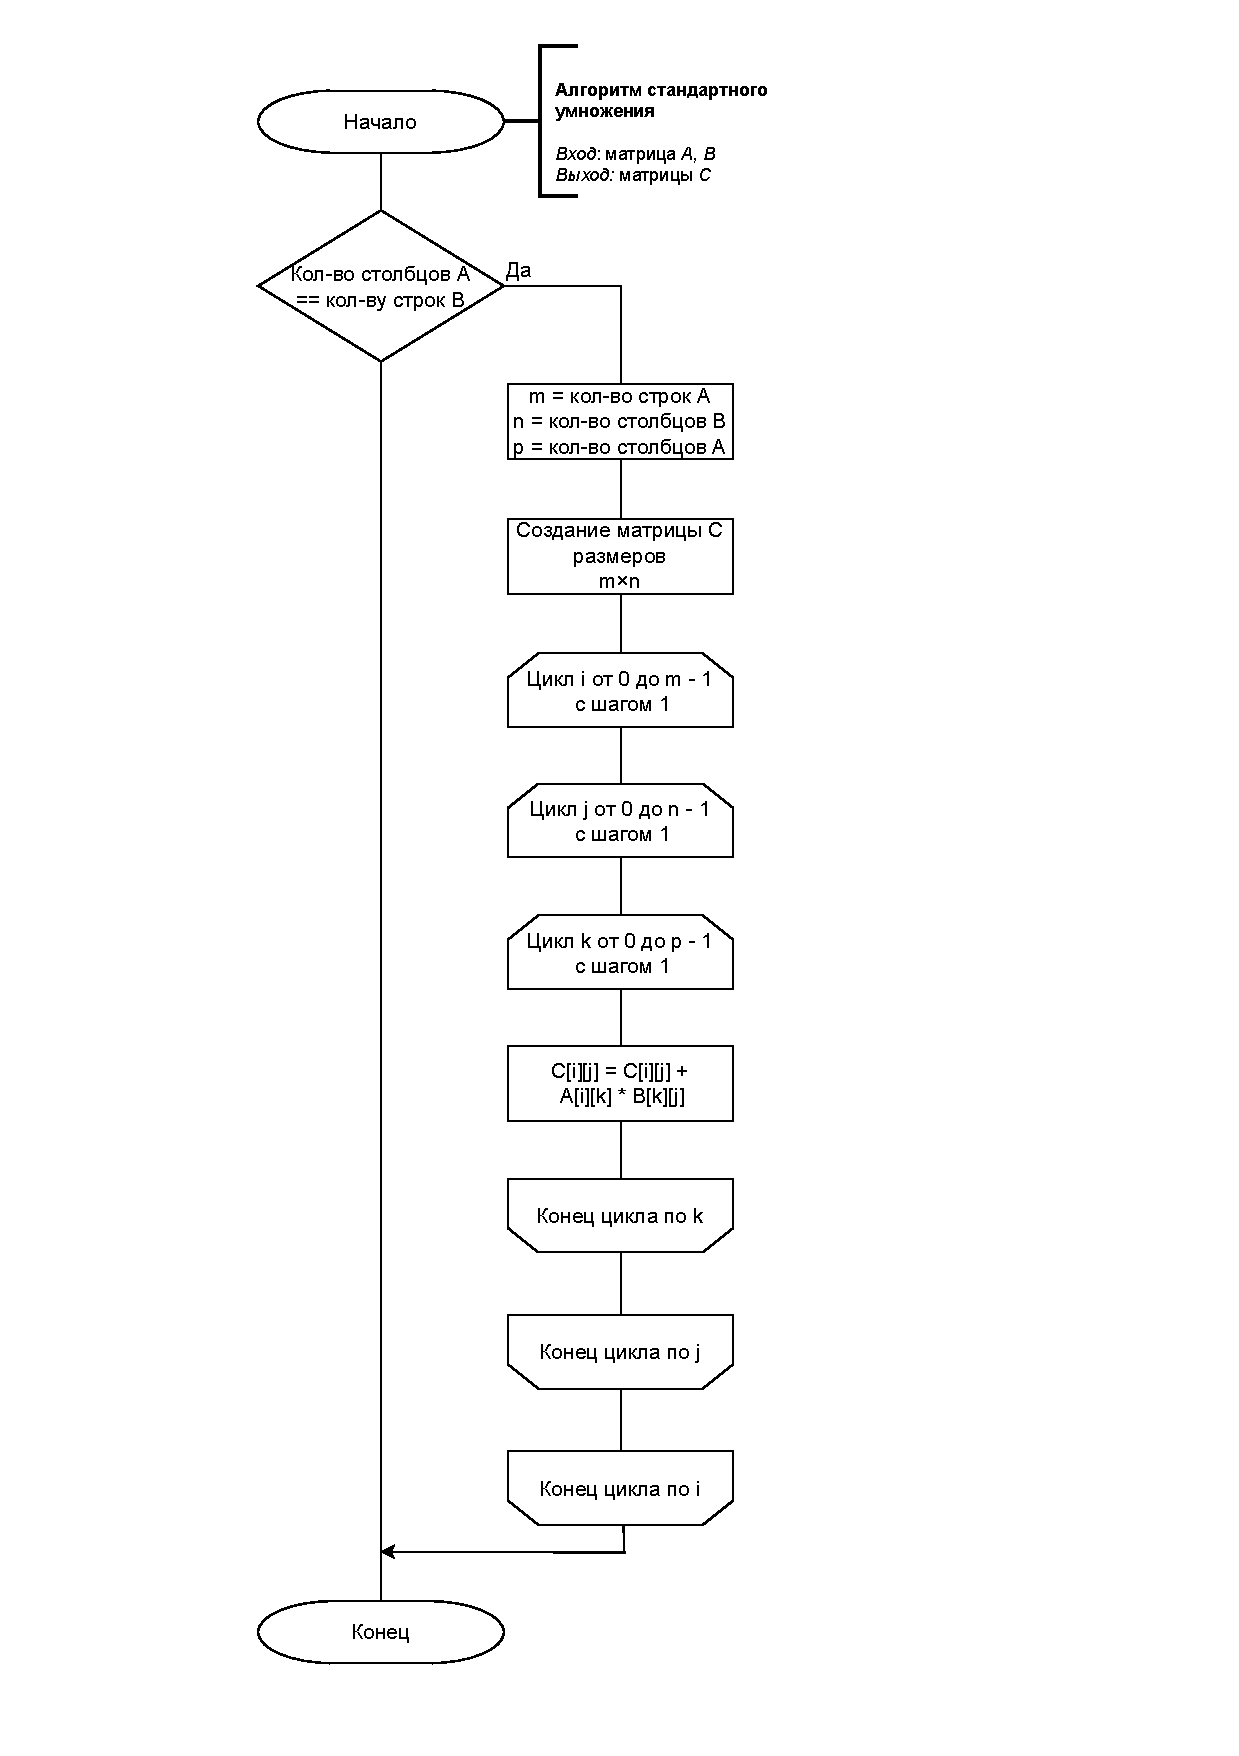
\includegraphics[height=0.9\textheight, page=1]{img/algorithms.pdf}
	\caption{Схема стандартного алгоритма умножения матриц}
	\label{fig:Stand}
\end{figure}

\clearpage

\begin{figure}[h]
	\centering
	\includegraphics[height=0.9\textheight, page=2]{img/algorithms.pdf}
	\caption{Схема алгоритма умножения матриц методом Винограда (начало)}
	\label{fig:Vinograd1}
\end{figure}

\clearpage

\begin{figure}[h]
	\centering
	\includegraphics[height=0.9\textheight, page=3]{img/algorithms.pdf}
	\caption{Схема алгоритма умножения матриц методом Винограда (конец)}
	\label{fig:Vinograd2}
\end{figure}

\clearpage

\begin{figure}[h]
	\centering
	\includegraphics[height=0.9\textheight, page=4]{img/algorithms.pdf}
	\caption{Схема оптимизированного алгоритма умножения матриц методом Винограда (начало)}
	\label{fig:VinogradOpt1}
\end{figure}

\begin{figure}[h]
	\centering
	\includegraphics[height=0.9\textheight, page=5]{img/algorithms.pdf}
	\caption{Схема оптимизированного алгоритма умножения матриц методом Винограда (конец)}
	\label{fig:VinogradOpt2}
\end{figure}

\clearpage

\section{Описание используемых типов данных}
При реализации алгоритмов будут использованы следующие структуры данных:

\begin{itemize}
	\item \textit{строка}~--- массив символов типа $wchar{\_}t$;
	\item \textit{длина строки}~--- целое число типа $int$;
	\item \textit{матрица}~--- двумерный массив значений типа $int$.
\end{itemize}

\section{Модель вычислений для проведения оценки трудоемкости алгоритмов}
Для последующего вычисления трудоемкости необходимо ввести модель вичислений:

\begin{enumerate}
	\item операции из списка %\ref{eq:operations1} имеют трудоемкость \textbf{1};
	\begin{equation}
		\label{eq:operations1}
		\begin{gathered}
			+, -, =, +=, -=, ==, !=, <, >, <=, >=, [], \\ ++, --, \&\&, >>, <<, ||, \&, |
		\end{gathered}
	\end{equation}
	\item операции из списка %\ref{eq:operations1} имеют трудоемкость \textbf{2};
	% \begin{equation}
	% 	\label{eq:operations2}
	% 	*, /, %, *=, /=, %=
	% \end{equation}
	\item Трудоемкость условного оператора:
	\item Трудоемкость цикла:
\end{enumerate}

\section{Трудоемкость алгоритмов}

\subsection*{Классический алгоритм}
\subsection*{Алгоритм Винограда}
\subsection*{Оптимизированный алгоритм Винограда}
	
\section*{Вывод}

В данном разделе на основе теоретических данных были перечислены требования к ПО, а также были построены схемы требуемых алгоритмов на основе теоретических данных, полученных на этапе анализа.